\documentclass[tikz]{standalone}

\pagestyle{empty}


\usepackage{amsmath}
\usepackage{tikz}
\usepackage{graphicx}
\usetikzlibrary{positioning,calc,fit,decorations.pathreplacing,arrows,positioning,backgrounds}

% Font settings:
\renewcommand{\familydefault}{\sfdefault}
\usepackage{pxfonts}
\newcommand{\figf}{\sffamily\bfseries\small} %Defines the font used for the labelling of figure panels.


% Color settings:
%\definecolor{hivc}{cmyk}{0,0.80,0.83,0.13}                %\definecolor{hivc}{HTML}{DE2D26}
\definecolor{hivc}{RGB}{24,116,205}
\definecolor{selfc}{cmyk}{0,0,0,0.6}                      %\colorlet{selfc}{gray!80!white}
\definecolor{Rblue}{RGB}{100,149,237}


\begin{document}
\scriptsize

\begin{tikzpicture}[anchor=north west]
\clip (0,0) rectangle +(18,-13);

\begin{scope}
	\begin{scope}
		\clip (0,0) rectangle +(11.5,-2);
		\node[anchor = north west] at (0.5,-0.3) {
			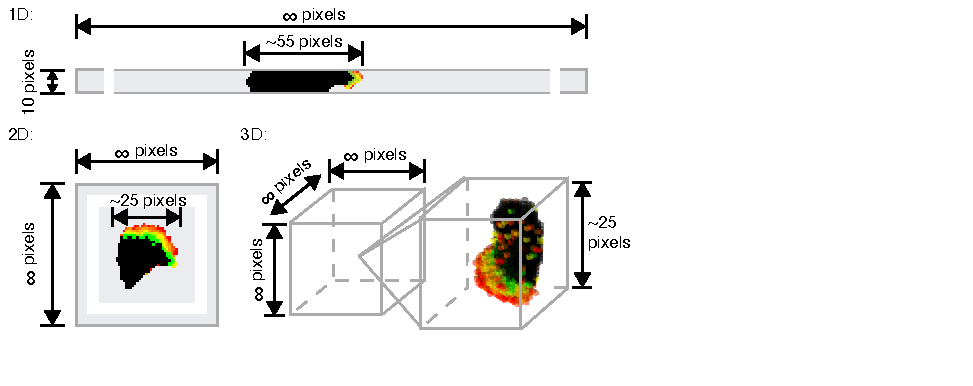
\includegraphics{../cartoons/all-setup.pdf}
		};
		
	\end{scope}
	
	\begin{scope}[xshift=12cm,yshift=0cm]
		\node[anchor = north west] at (0,-0.95){
			
\includegraphics{../cartoons/gradient.pdf}
		};
		\node[anchor = north west] at (0.1,-0.65) {activity:};
		\node[anchor = north west] at (0.1,-1.45) {0};
		\node[anchor = north west] at (1.15,-1.45) {max\textsubscript{act}};
	\end{scope}
	
	
	\node[anchor = north west] at (0,0) {\figf A};
\end{scope}

\begin{scope}[yshift=-2.1cm] % x 11.7
	\node[anchor = north west] at (0,-0){
		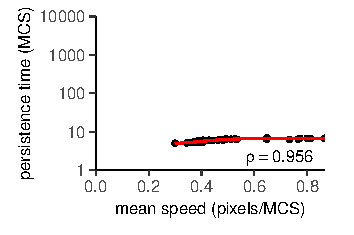
\includegraphics{../plots/F2panelB-1D.pdf}
	};
	%\node[anchor = north] at (4,-0.6) {1D};
	%\node[anchor = north west] at (0.3,-4.7){
%		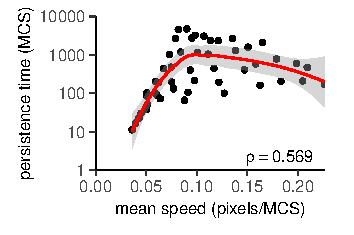
\includegraphics{../plots/F2panelB-2D.pdf}
%	};
%	\node[anchor = north] at (4,-4.6) {2D};
%	\node[anchor = north west] at (0.3,-8.7){
%		\includegraphics{../plots/F2panelB-3D.pdf}
%	};
%	\node[anchor = north] at (4,-8.6) {3D};
	\node[anchor = north west] at (0,-0.3) {\figf B};
\end{scope}



\begin{scope}[xshift = 6.3cm, yshift=-2.1cm]

	\node[anchor = north west] at (0,0){
		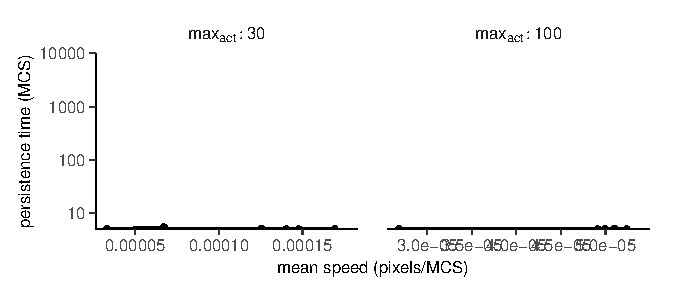
\includegraphics{../plots/F2panelC.pdf}
	};
	\draw[->, line width = 0.2mm] (4.45,-1.95) -- +(0.8, 0.4);
	\node[anchor = south west, rotate = 30] at (4.5,-1.9) {$\lambda$\textsubscript{act}};


	\node[anchor = north west] at (0,-0.3) {\figf C};
\end{scope}

\begin{scope}[yshift=-7cm]

	\node[anchor = north west] at (0,0){
		\includegraphics{../../phase-diagram/plots/phase-diagram.pdf}
	};
	\node[anchor = north west] at (8.7,-0.5){
		\includegraphics{../../phase-diagram/plots/dx-insets.pdf}
	};
	
	

	\node[anchor = north west] at (0,0) {\figf D};
\end{scope}


\end{tikzpicture}




\end{document}
